% !TeX spellcheck = en_US
\section{System Architecture}
\noindent A graphical representation of the system architecture can be seen in figure \ref{fig:architecture}.

\begin{figure}[H]
	\centering
	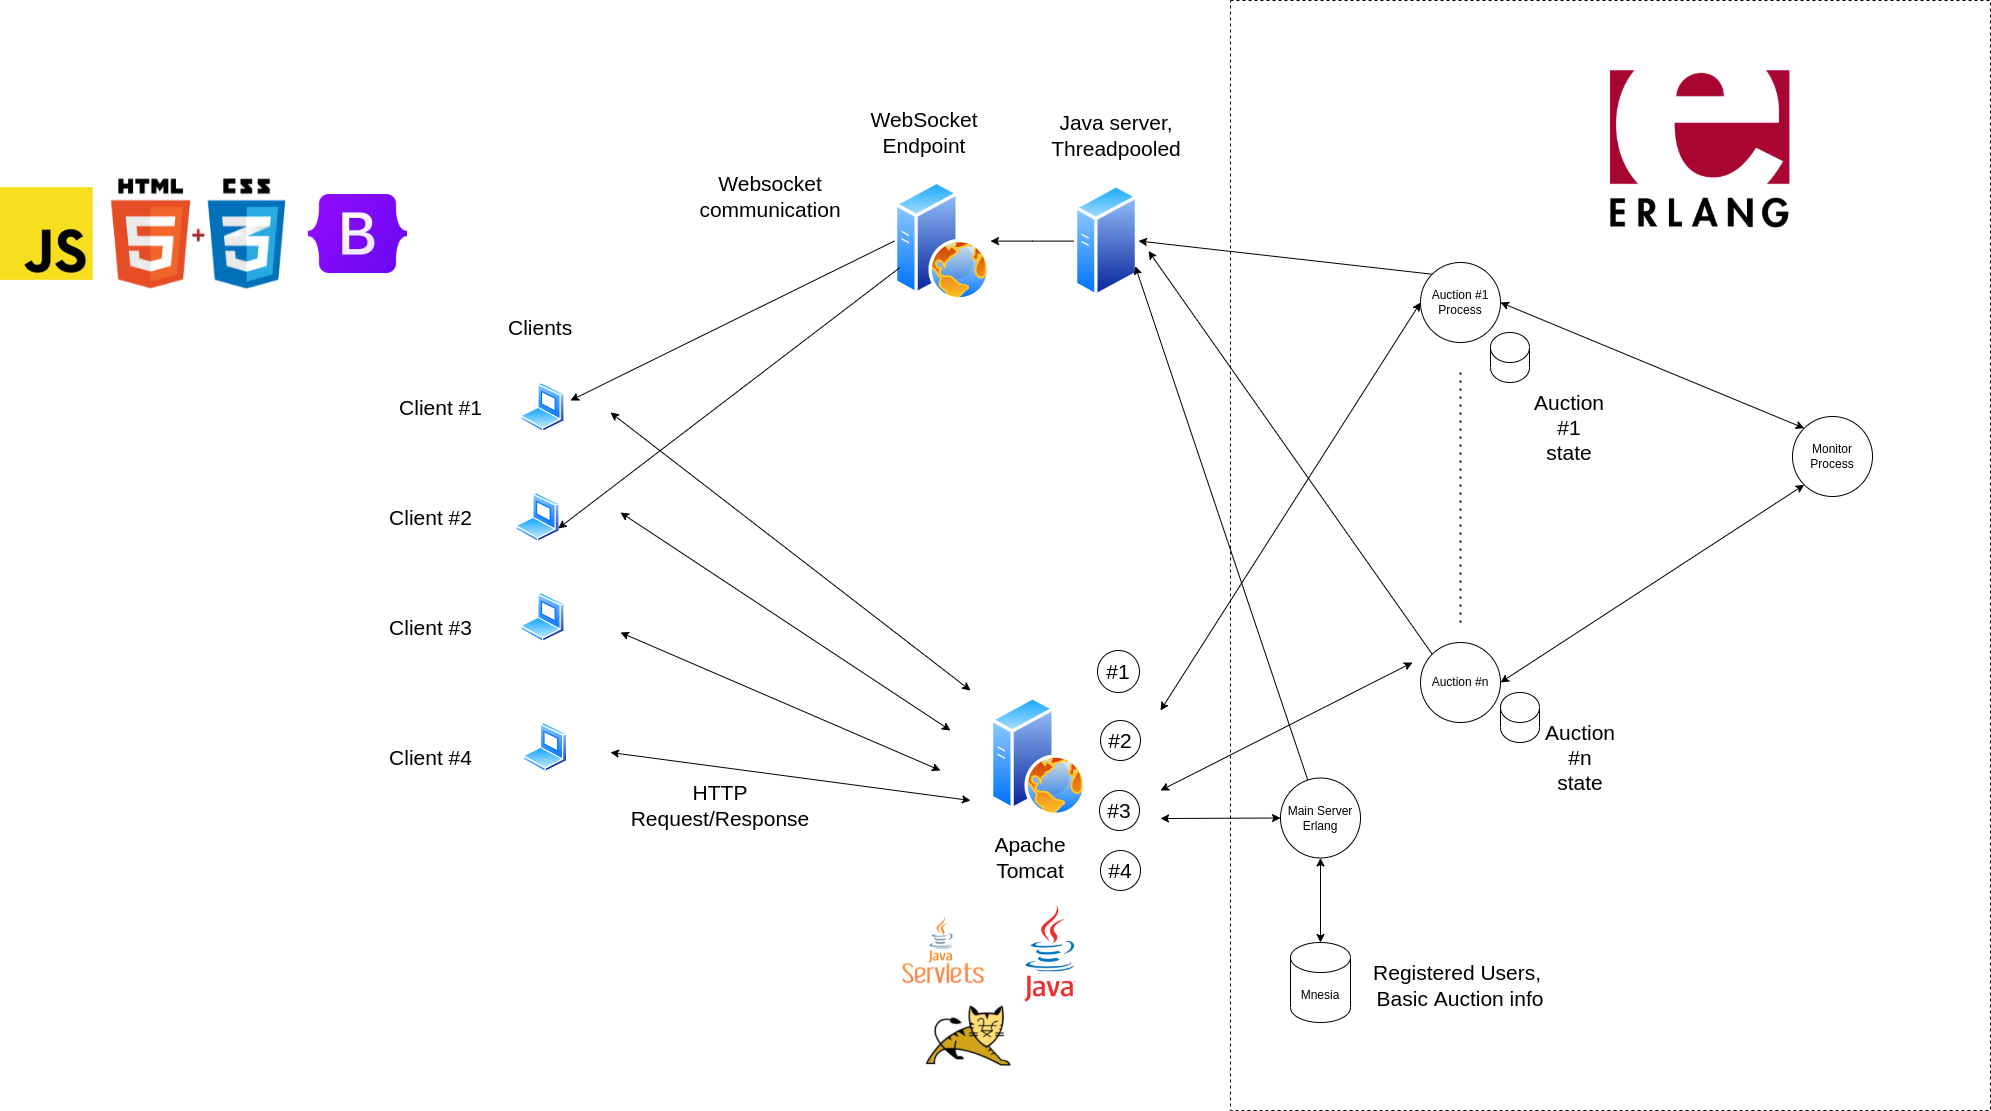
\includegraphics[width=1\linewidth]{img/systemStructure.png}
	\caption{System Architecture graphical representation}
	\label{fig:architecture}
\end{figure}

\noindent We can divide the overall system in two part:
\begin{itemize}
	\item The server side part: developed in Erlang, it is in charge of handling the request coming from the users and it has to handle the auctions and to maintain the global view of an auctions consistent among the users.
	
	\item The client side part: depeloved in Java, using EJB e JSP, and in Javascript for what regards the websocket. It is in charge of retrieving information from the server, create the GUI, update the GUI in order to let the user have a consistent view of the state of the auction and of the overall system.
\end{itemize}

\subsection{Server Side}

\subsubsection{Main Server}

\subsubsection{Auction Handler}

\subsubsection{Monitor And Supervisor}

\subsection{MnesiaDB}

\subsection{Client Side}

\subsection{Synchronizations Issues}